   
\section{Methods}
In this section, we propose a non-parametric model based on quantile regression to model backfill patterns and introduce the covariates that help capture the backfill dynamics across time. 

\subsection{Real-Time Quantile Regression}

For any test date $S$, we are trying to make distributional projection of $Y_{itL}$ for all $t \in [S-L, S)$. We use the notation $Q_{Y_{itL}|X_{itl}}^{\tau}$ to represent the $\tau$th quantile of $Y_{itL}$ given $X_{itl}$, where $X_{itl}$ is the vector of features based on $\{y_{itl}\}_{t+l\leq s}$. 
$$Q_{Y_{itL}|X_{itl}}^{\tau} = \inf \{y: F_{Y_{itL}|X_{itl}}(y) \geq \tau\}$$
Motivated by reducing the relative error between the projections and the target, we do a log transformation (natural logarithm) $f(x) = log(x + a)$ of all the variables. $a$ is a small enough constant to avoid invalid values. Since $f(\cdot)$ is monotonically increasing, 
$$ Q_{f(Y_{itL})|X_{itl}}^{\tau} = f(Q_{Y_{itL}|X_{itl}}^{\tau}) $$
We now make the assumption that the $\tau$th conditional quantile on log scale is given as a linear function of explanatory variables.

$$Q_{f(Y_{itL})|f(X_{itl})}^{\tau}= \beta^{\tau T}X_{itl}$$
The covariates included in $X_{itl}$ are the following:
\begin{itemize}
    \item $\mathbbm{1}(\mbox{wd}(t+l) == k)$: indicator functions checking the day-of-week of the report date $t+l$, where $k \in \{0, 1, 2, ..., 5\}$. 
    \item $\mathbbm{1}(\mbox{wd}(t) == k)$ : indicator functions checking the day-of-week of the report date $t$, where $k \in \{0, 1, 2, ..., 5\}$.
    \item $\mathbbm{1}(\mbox{mw}(t+l) == k)$ : indicator functions checking the week-of-month of report date $t+l$, where $k \in \{0, 1, 2, ...,3\}$
    \item $f(\widetilde{y}_{itl})$: average of 7-day past values on log scale.
    \item $\mathbbm{1}(\sqrt{y_{itl}} \in \mbox{interval}_k)$ where $\mbox{interval}_k$ are uniform bins at square-root level
    \item \mbox{7day-slope}: $f(\widetilde{y}_{itl}) - f(\widetilde{y}_{i(t-7)(l+7)})$ : the 7-day slope, where we compare the difference between the 7-day average of current observations and the 7-day average of the observation assigned to 7 days ago on log scale.
    \item 7day-Modification where we compare the difference between the 7-day average of the current raw counts and the 7-day average from the first release. 
    $$\mbox{7day-Mod} = f( \widetilde{y}_{itl}) - f(\widetilde{y}_{it0})$$
    \item 7day-Prev-Mod-start where we compare the difference between the 7-day average of the raw counts reported a week ago with the same lag and the 7-day average of the raw counts reported a week ago from the first release. 
    $$\mbox{7day-Prev-Mod-Start} = f( \widetilde{y}_{i(t-7)l}) - f(\widetilde{y}_{i(t-7)0})$$
    \item 7day-Prev-Mod-follow 
    $$\mbox{7day-Prev-Mod-Follow} = f(\widetilde{y}_{i(t-7)l}) - f( \widetilde{y}_{i(t-7)(l+7)})$$

\end{itemize}
$\mbox{wd}(\cdot)$ is a function returning the day of the week as integers, where Monday is 0 and Sunday is 6. $\mbox{mw}(\cdot)$ is a function checking the week of a month. For example, $\mbox{mw}(\cdot) = 0$ represents the first week of a month that starts from a Sunday. $\widetilde{y}_{itl} = \sum_{v=1}^7 y_{i(t-v)(l+v)}$ is the average of 7-day past values reported at the same date $t+l$

We achieve the estimates of coefficients by solving the problem
$$ \beta^{\tau} = \arg\min_{\beta} \sum_{l\in \mathcal{L}, t+l < S}(\rho_\tau (f(Y_{itL}) - X_{itl}\beta)) + \lambda ||\beta||_1$$

where $\rho$ is the quantile loss\cite{Koenker1978}, $\mathcal{L} = \{l: 0 \leq l \leq L\}$. $||\cdot||_1$ is the $\mathcal{l}_1$ norm. The hyper-parameter $\lambda \geq 0$ controls the complexity of the model. 


The model is trained adaptively. At each test date $S$, a series of new observations is reported which gives a series of $y_{itl}$s,

$$y_{i}^S = \{\underbrace{y_{i,S,0}, y_{i, (S-1), 1}, y_{i, (S-2), 2}, \cdots, y_{i, (S -L +1),(L-1)}}_\text{Testing Data}, \underbrace{y_{i, (S-L), L}}_\text{Target},  \cdots \}$$.
Note that, the backfill sequence of $y_{i(S-L)}$ is moved from testing to training since the target $y_{i,(S-L), L}$ becomes available. 

\begin{figure}
    \centering
    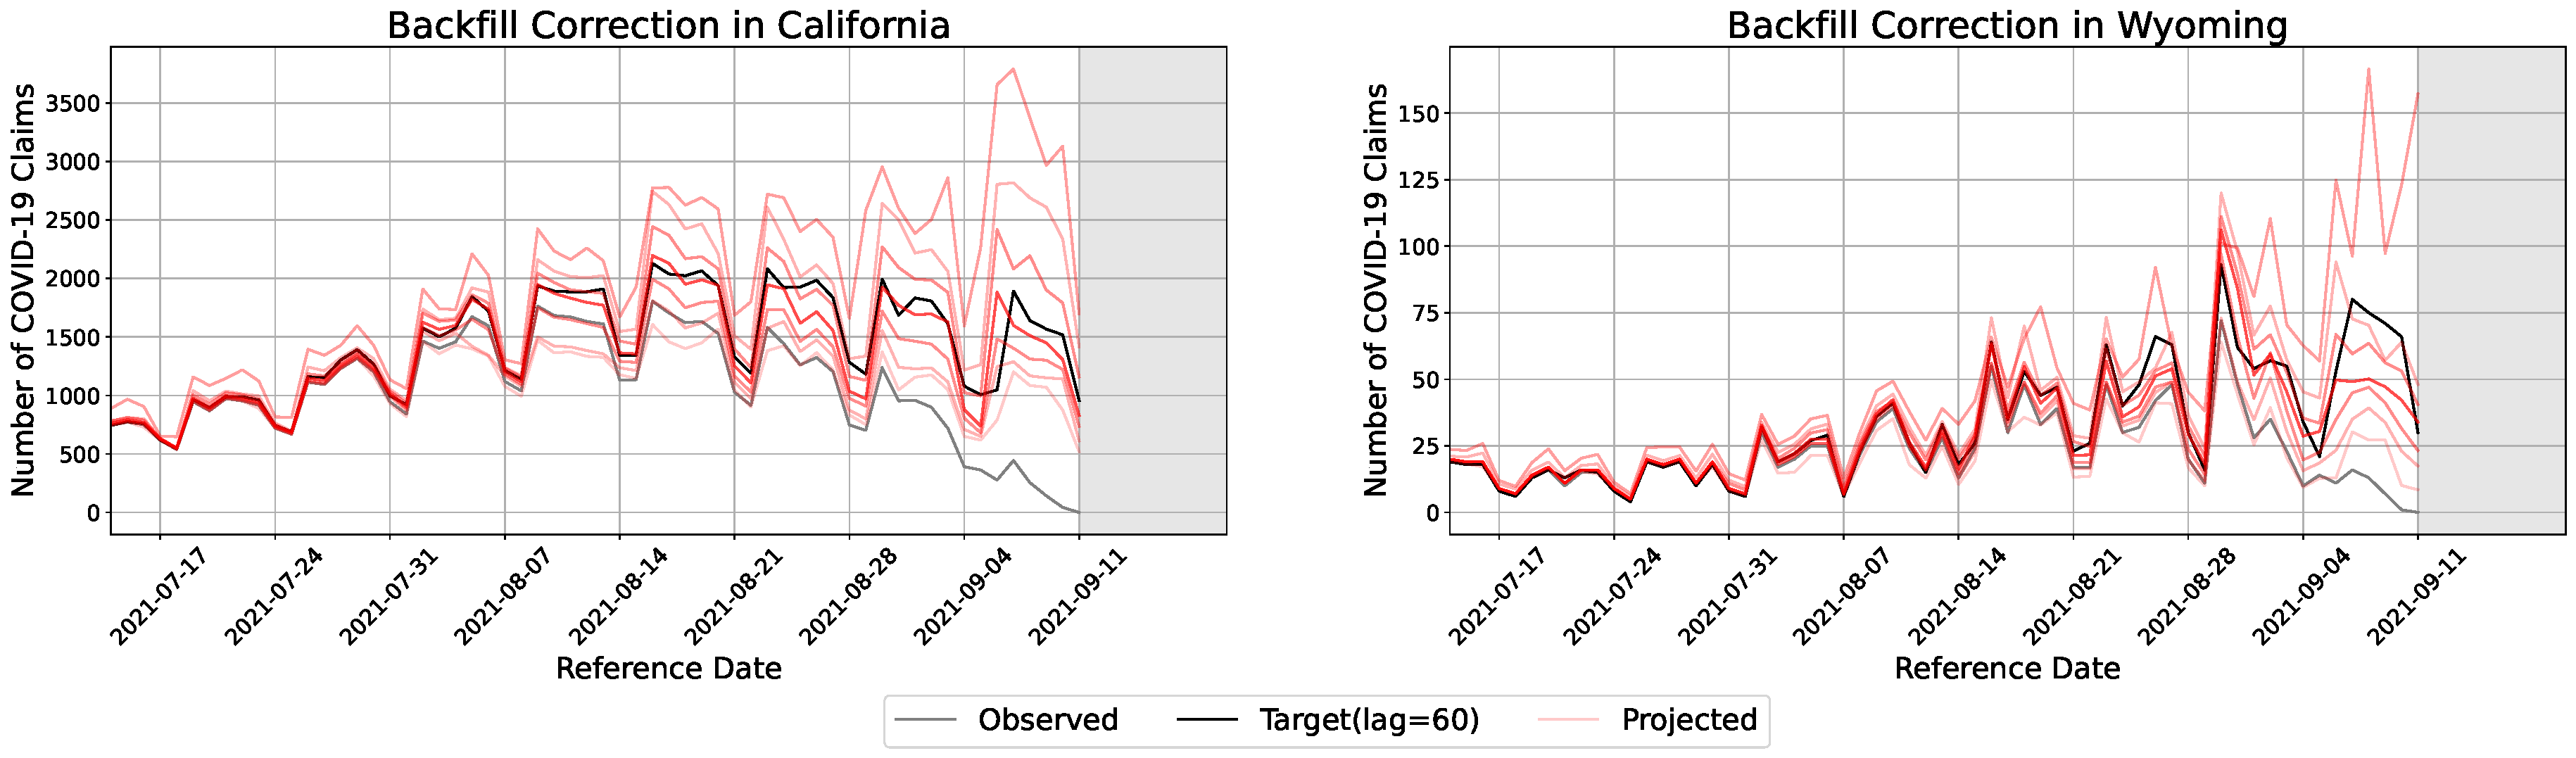
\includegraphics[width=\textwidth]{figs/count_pred_example_ca&wy.pdf}
    \caption{\textit{Illustration of estimating target number of CHNG outpatient COVID-19 claims as of 2021-09-11. The gray curve shows the most recent release of the number of COVID claims based on CHNG outpatient data in California and Wyoming. The red lines show the projected quantiles of the 60th revision of the number of COVID-19 claims for each reference date. The black curve shows the actual 60th revision for the values of each reference date in the future.}}
\end{figure}

\textbf{Shortening the Lag Window}
%% TODO: add a figure to explain it. Some kind of diagram? 
As the backfill patterns vary largely over lags, we investigate shortening the lag window in the regularized backfill correction problem and train separate models for observations with different levels of lag. Theoretically, training separate models is the same as training one model with all data pooled together but incorporating indicators to inform the level of lag (The only difference is that, fitting separately generates different variance estimates) in linear regression. However, it is not the case when lasso penalty is added for reducing the complexity of the model and rolling out extreme outliers. When making projection of $y_{itl'}$($l'$ is small enough, e.g. $l' \leq 7$), instead of using all the data as described above, we now change the problem to be
$$ \beta^{\tau} = \arg\min_{\beta} \sum_{l\in \mathcal{L}, t+l < S}(\rho_\tau (f(Y_{itL}) - X_{itl}\beta)) + \lambda ||\beta||_1$$
where $\mathcal{L}^(l') = \{l: l'-c \leq l \leq l'+ c\}$. The length lag window for this training is $2c +1$. Shortening the training window is not computationally advantageous since more models need to be trained, but the projection performance will be changed.

\textbf{Adjusting weights of Observations} The observations are not equally useful when estimating the backfill patterns. Weights are leveraged to observations as follow:
$$ \beta^{\tau} = \arg\min_{\beta} \sum_{l\in \mathcal{L}, t+l < S}w(\rho_\tau (f(Y_{itL}) - X_{itl}\beta)) + \lambda ||\beta||_1$$
where $w = \exp(-\gamma \cdot D_s \cdot D_y)$. $D_d$ and $D_y$ are two variables that affect weighting from different aspects. For each obervation $y_{itl}$, $D_d = S - (t+l)$ measures the \textit{freshness}, $D_y = \widetilde{y}_{i,(S),0} - \widetilde{y}_{itl}$ measures the similarity to the most up-to-date report. The hyper-parameter $\gamma \geq 0$ controls the additional $focus$ that we put on recent data. 

%% TODO
In general, there are three hyper-parameters to tune in practice:1) $c$ for controlling the training lag window ; 2) $\lambda$ for the lasso penalty; 3) $\gamma$ for controlling the weights of observations. Figure X1 and X2 shows the (not that confident about how to explain this part or are the figs currently good enough? )

\begin{figure}
    \centering
    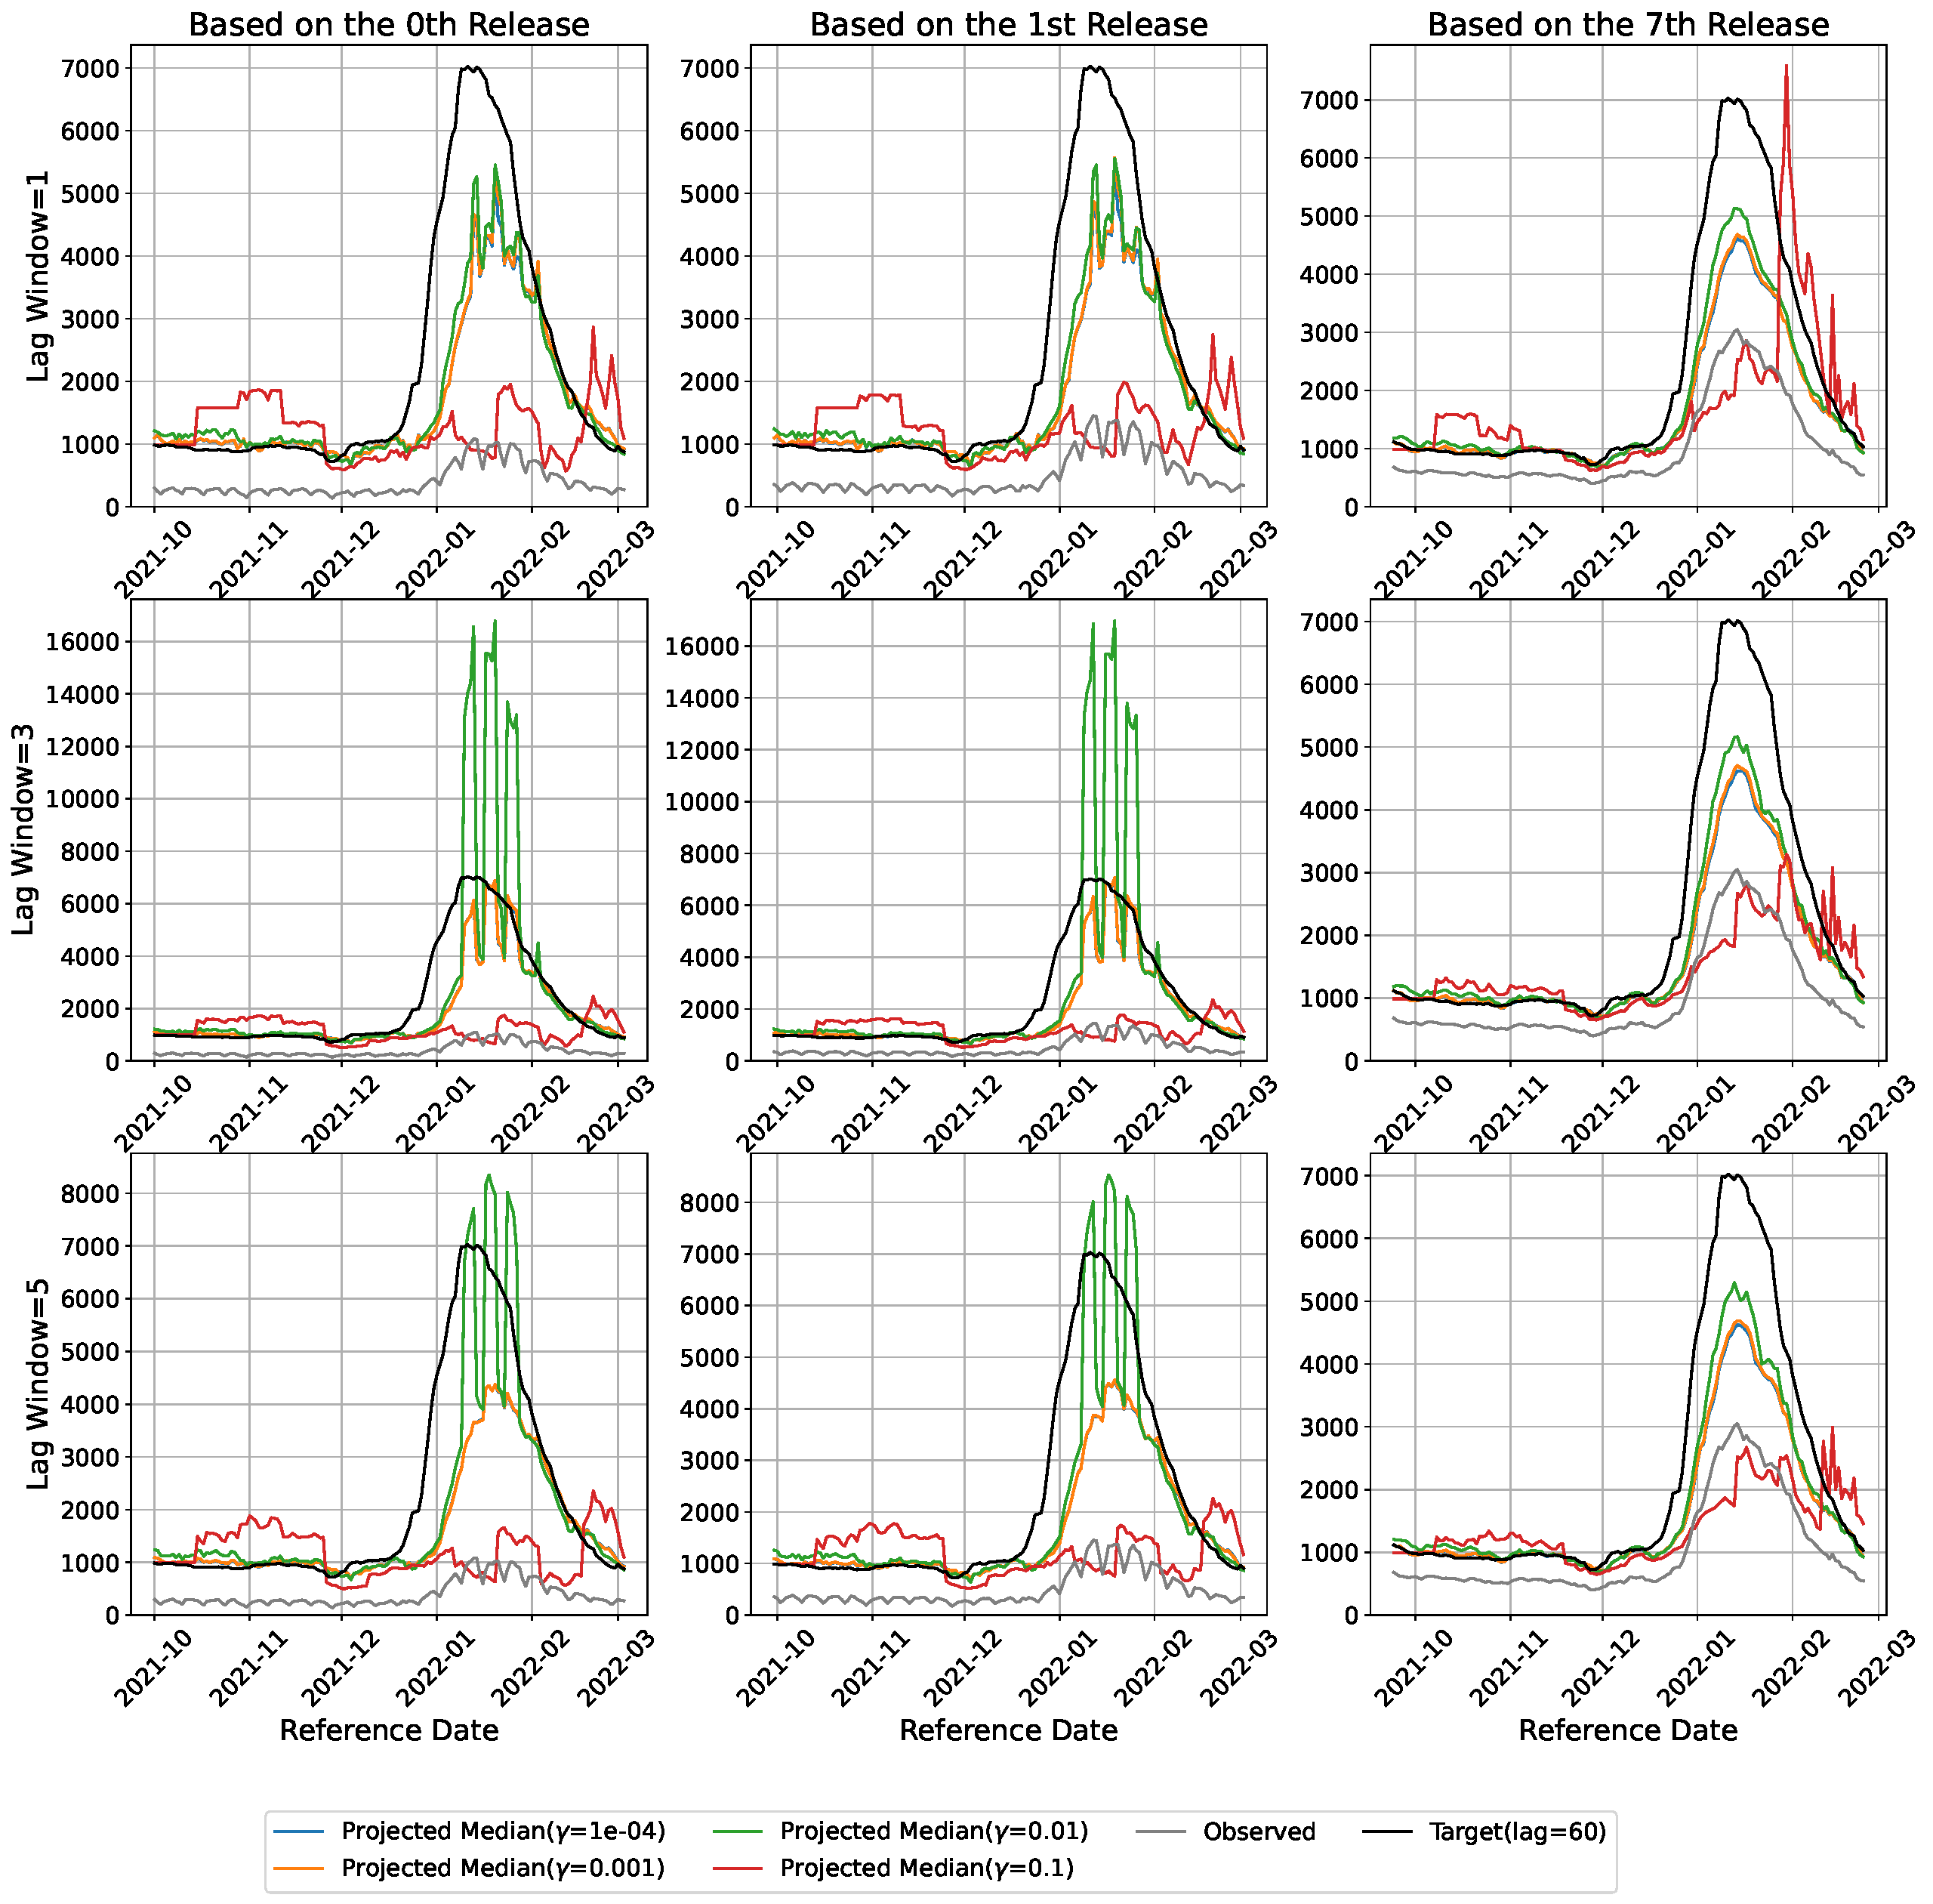
\includegraphics[width=\textwidth]{figs/count_pred_gamma_lagpad_tuning_ca_new_covs_added.pdf}
    \caption{\textit{}}
\end{figure}

\begin{figure}
    \centering
    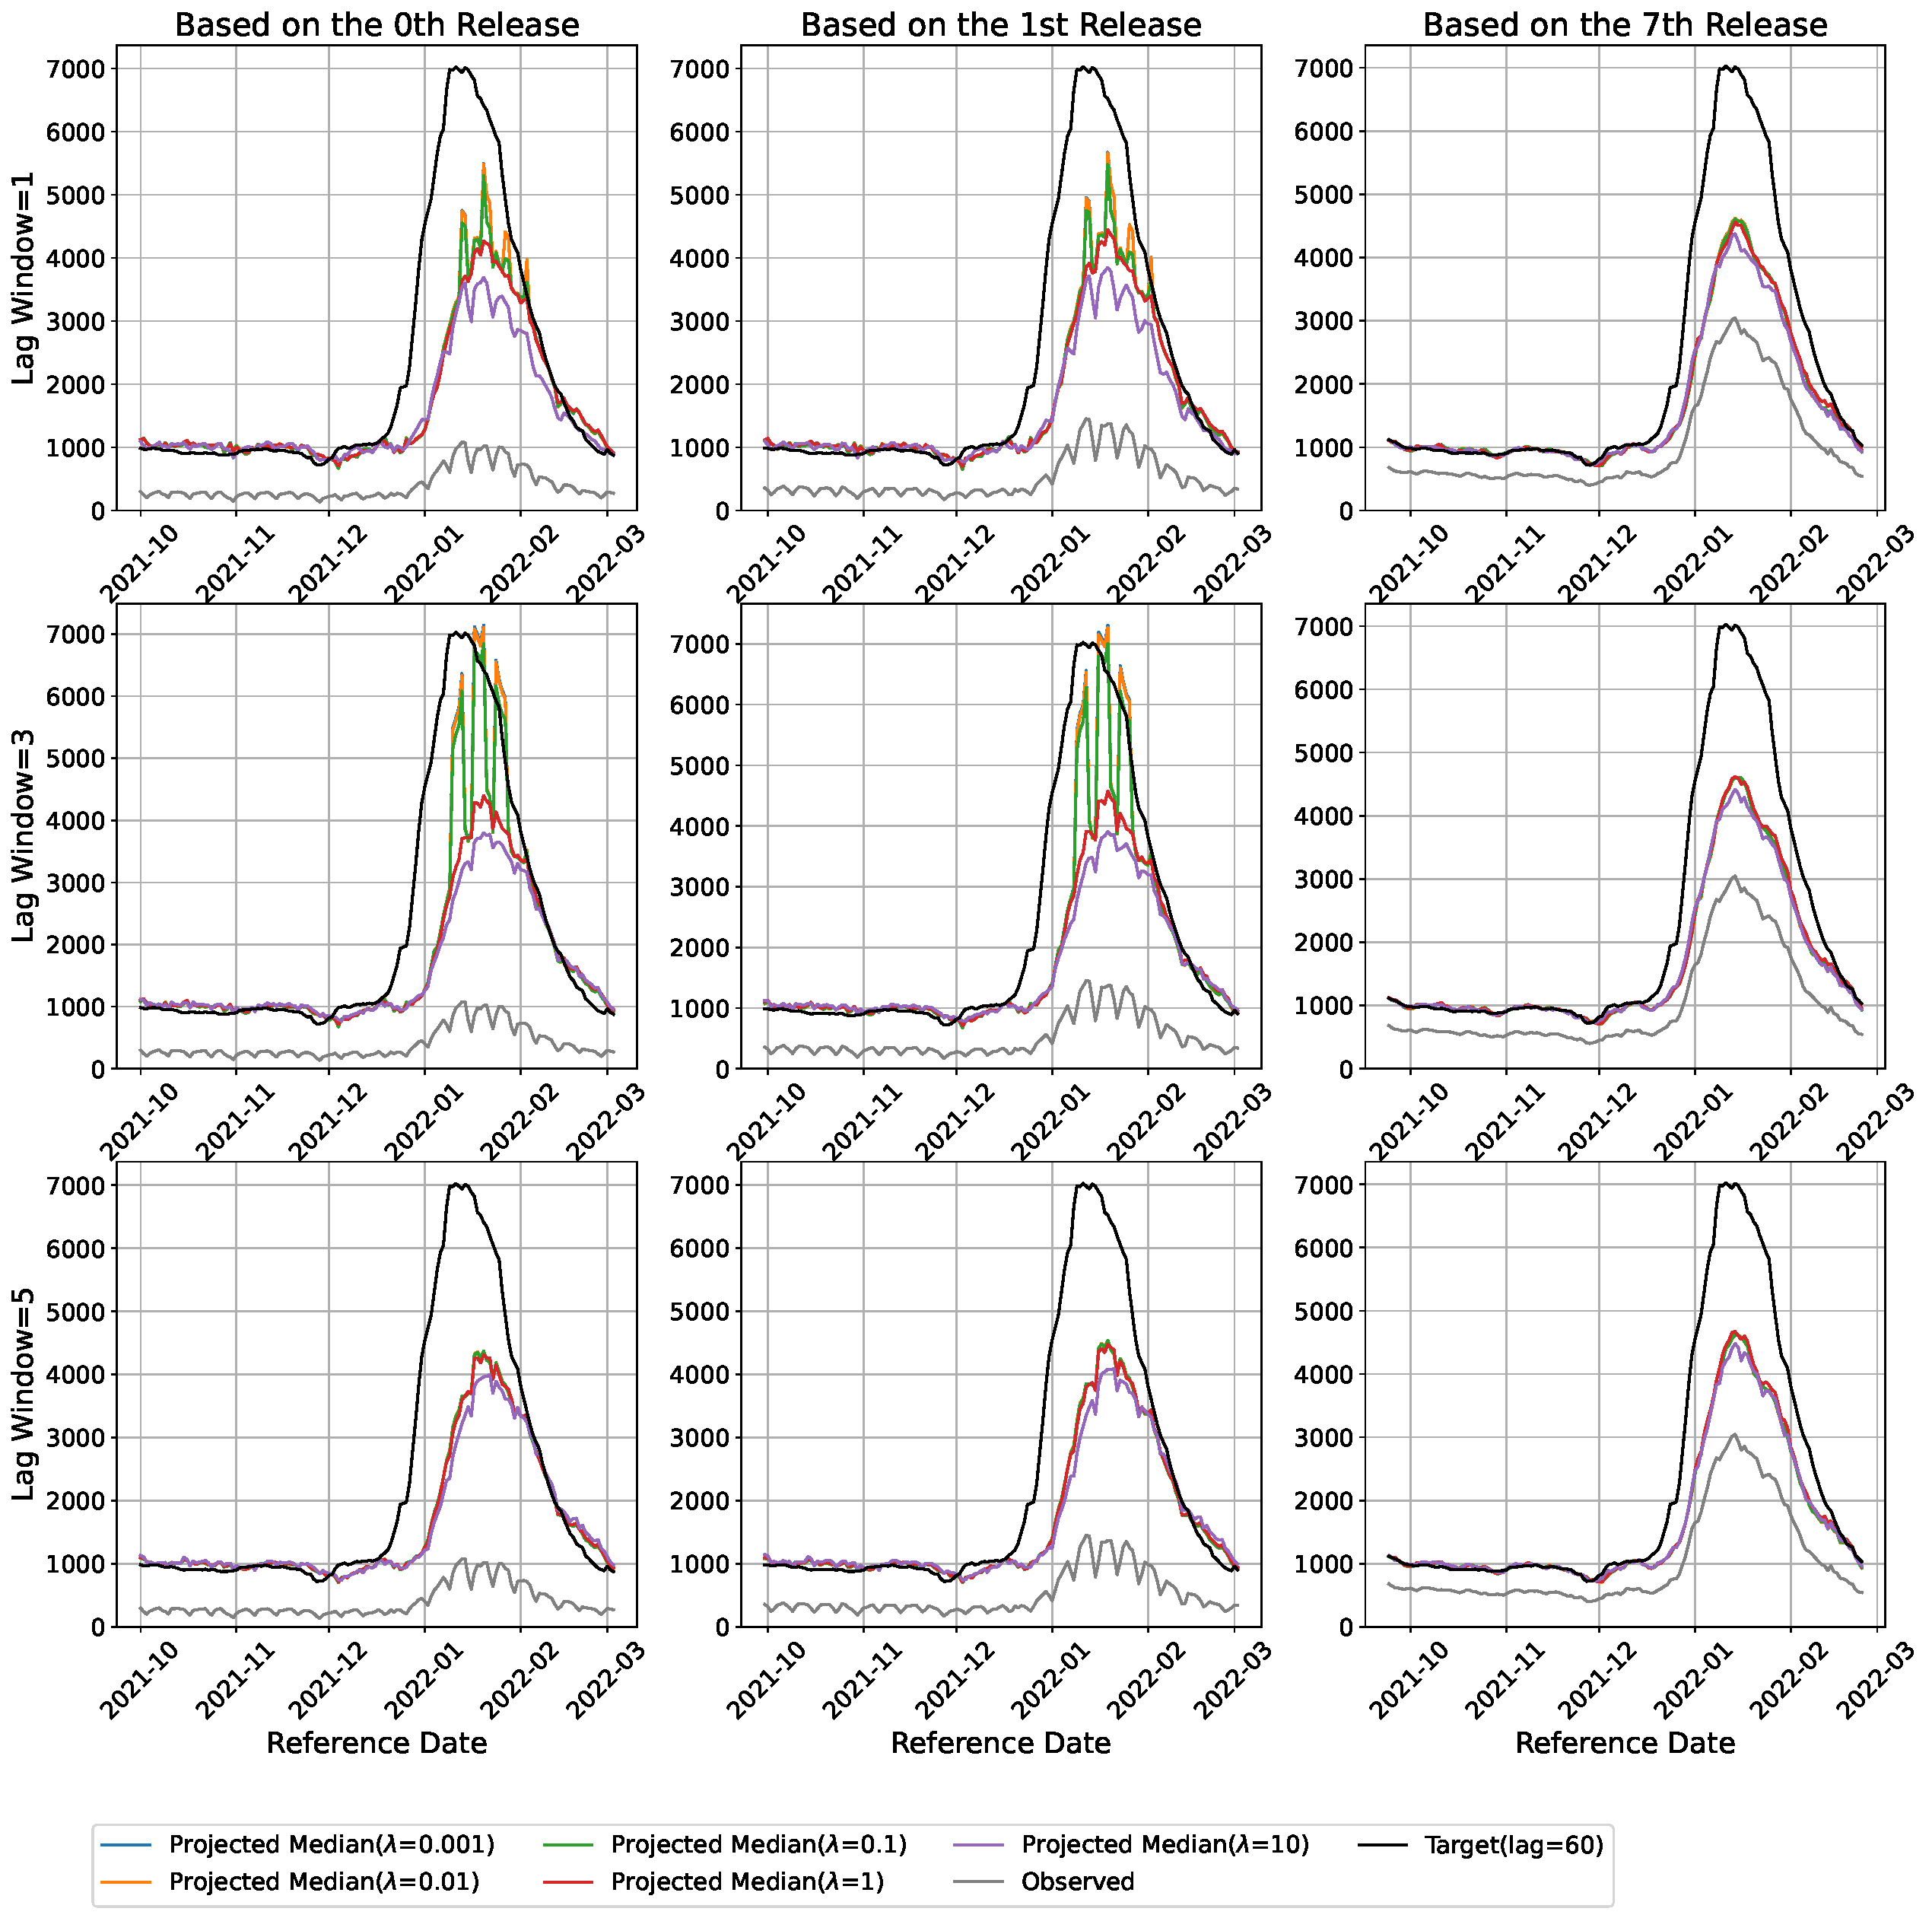
\includegraphics[width=\textwidth]{figs/count_pred_lambda_lagpad_tuning_ca_new_covs_added.pdf}
    \caption{\textit{}}
\end{figure}

\subsection{Incorporating Fraction Adjustment for Fraction Projection}
Turning our focus now to fraction projection. Different from counts projection where zeros are simply filled with missingness when there is no update provided yet, the edge cases for fraction projection is more complicated to dealing with. We mainly suffer from two cases: 1) fraction with extremely small denominators (can even be zeros) which means the revision of numerators is faster than that of denominators. This can result in incredibly large fraction observations. Such fractions are not statistically representative and mostly exist when lag is super small; 2) fraction equals to zero. The log transformation $f(\cdot)$ proposed in the previous section are no longer suitable for this case since fractions are already small enough. Inappropriately large constant $a$ can introduce noise into the data\cite{Bosse2023}. 

Here we propose a Beta prior approach based on a $\mbox{lag}^{-1}$ model, which can also serve as a baseline model. The make all the observations valid fractions, we add 1 and 100 respectively to the numerators and denominators beforehand. For location $i$, at test date $S$, consider the model below

$$Q_{f(Y_{itL})|f(X_{itl})}^{\tau}= \beta^{\tau T}X_{itl}$$

Covariates included in $X_{itl}$ are the following:

\begin{itemize}
    \item $\mathbbm{1}(\mbox{wd}(t+l) == k)$: indicator functions checking the day-of-week of the report date $t+l$, where $k \in \{0, 1, 2, ..., 5\}$. 
    \item $\mathbbm{1}(\mbox{wd}(t) == k)$ : indicator functions checking the day-of-week of the report date $t$, where $k \in \{0, 1, 2, ..., 5\}$.
    \item $\mathbbm{1}(\mbox{mw}(t+l) == k)$ : indicator functions checking the week-of-month of report date $t+l$, where $k \in \{0, 1, 2, ...,3\}$
    \item $f(\widetilde{y}_{itl})$: average of 7-day past values on log scale.

\end{itemize}

\begin{figure}
    \centering
    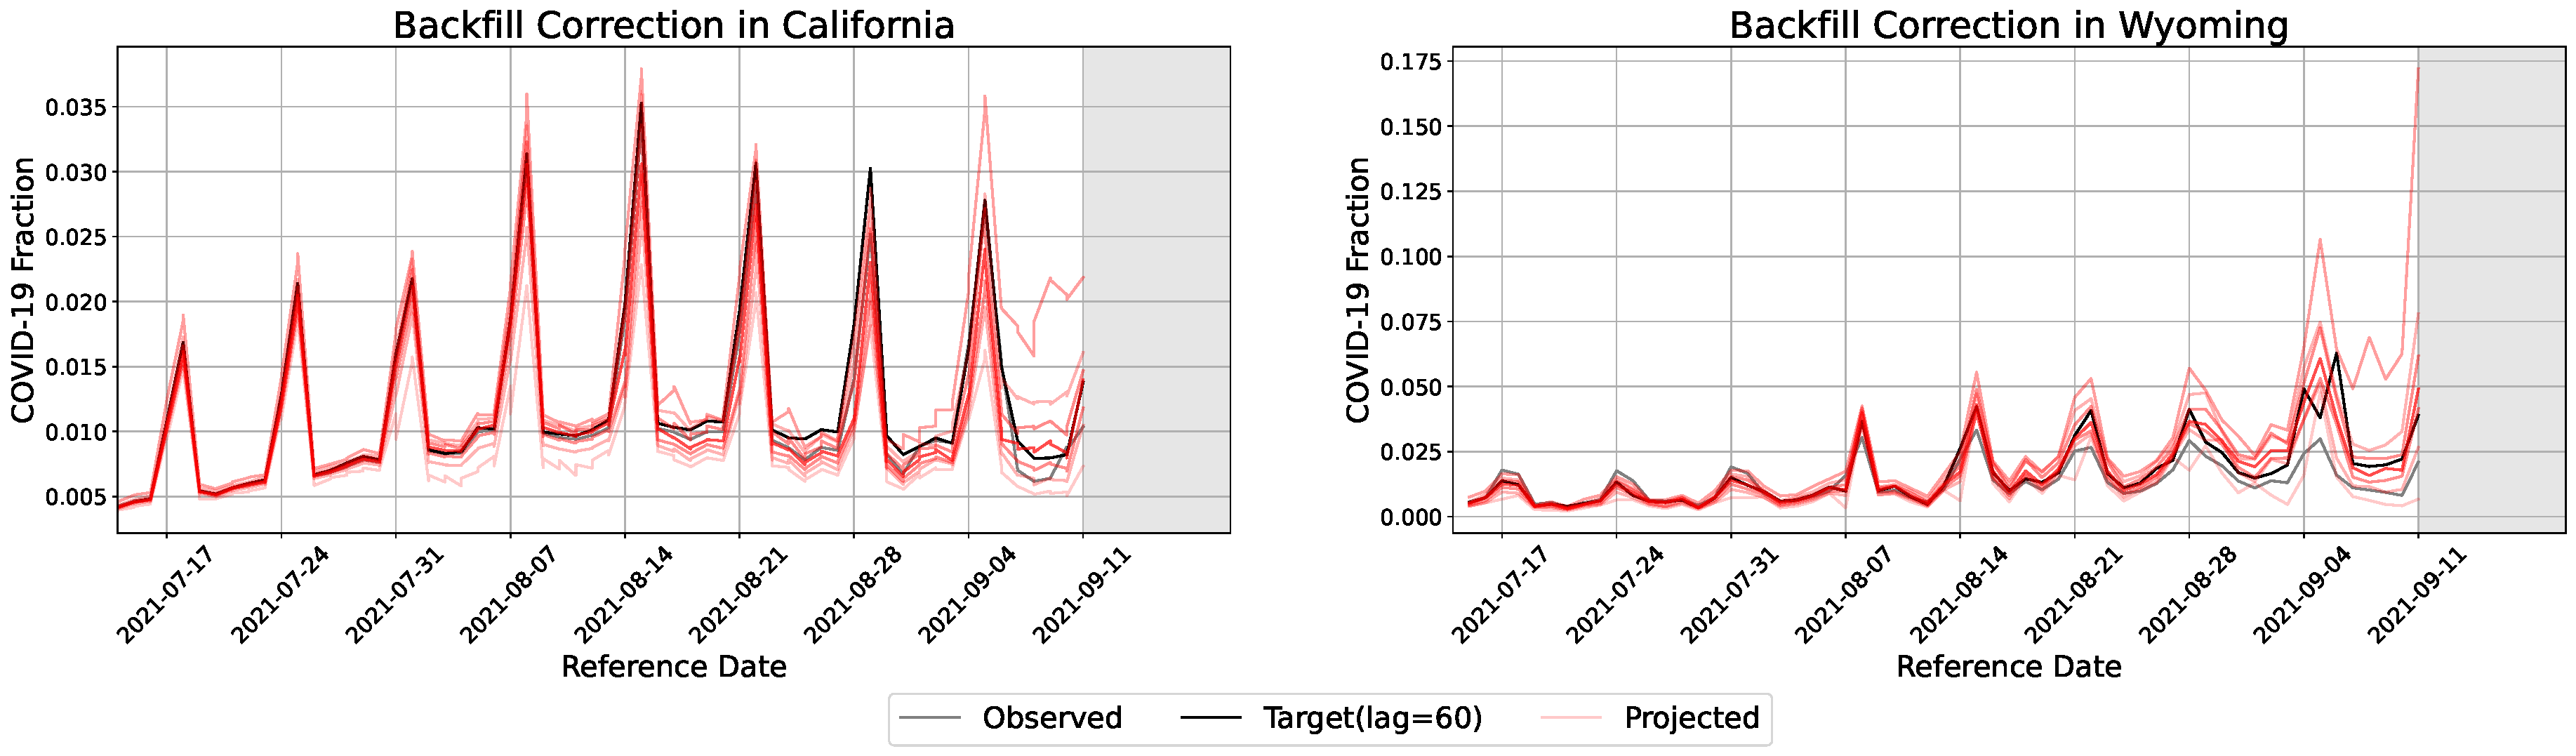
\includegraphics[width=\textwidth]{figs/fraction_pred_example_ca&wy.pdf}
    \caption{\textit{Illustration of estimating target of CHNG outpatient COVID-19 fractions as of 2021-09-11. The gray curve shows the most recent release of the COVID fractions based on CHNG outpatient data in California and Wyoming. The red lines show the projected quantiles of the 60th revision of the COVID-19 fractions for each reference date. The black curve shows the actual 60th revision for the values of each reference date in the future.
}}
\end{figure}

We assume that $Y_{itl}|X_{itl}$ follows Beta distribution that are day-of-week specific. For each day of a week, the predicted quantiles of $y_{itl}$ on log scale are exponentiated and utilized to estimate the parameters $\alpha$ and $\beta$ of the Beta distribution using Non-Linear Minimization\cite{Dennis1983}\cite{Schnabel1985}. And then,  
$$\mbox{Pseudo Numerator} = \alpha$$
$$\mbox{Pseudo Denominator} = \alpha + \beta$$
$$y_{itl} = \frac{\mbox{num}_{itl}}{\mbox{denom}_{itl}} \rightarrow \frac{\mbox{num}_{itl} + \alpha}{\mbox{denom}_{itl} + \alpha + \beta}$$
This adjustment is applied not only to $y_{itl}$ but also to all corresponding covariates. 

